\chapter{Solu\c{c}{\~a}o proposta}\label{CAP_SOLUCAOPROPOSTA}
\begin{flushright}
	\textit{``Poder é sempre perigoso. Atrai o pior e corrompe o melhor. Nunca pedi por poder. Poder só é dado para aqueles que estão dispostos a abrir mão de si por ele.''\\
			(Ragnar Lothbrok)}
\end{flushright}

Este capítulo descreve a solução proposta para o problema de recomendar atividades em workflows científicos, que utiliza uma ontologia de domínio e frequência de atividades para recomendar atividades para cientistas durante a construção de \emph{workflows} científicos. Também são descritas as soluções propostas para o uso de classificadores e regressores para resolver o problema de recomendação de atividades, bem como o uso de um classificador composto e um \emph{ensemble} de classificadores.

Primeiramente será detalhado como a ontologia foi construída, qual a metodologia foi usada e o processo de sua construção. Em seguida será detalhado o conjunto de dados, como foram obtidos, sua organização em um modelo relacional e como ocorreu a modelagem desses dados para solucionar o problema de recomendação. O próximo passo é explicar as alterações necessárias nos dados para serem usados por classificadores e regressores. Em seguida, será explicada a estratégia de validação dos experimentos. Por fim, na última seção do capítulo, será detalhada a solução proposta que utiliza a ontologia construída.
 \usepackage[utf8]{inputenc}		% Codificacao do documento (conversão automática dos acentos)
 \usepackage{lastpage}			% Usado pela Ficha catalográfica
 \usepackage{indentfirst}		% Indenta o primeiro parágrafo de cada seção.
 \usepackage{color}				% Controle das cores
 \usepackage{graphicx}			% Inclusão de gráficos
 
 \usepackage{microtype} 			% para melhorias de justificação
 \DisableLigatures{encoding = *, family = *} %Remove ligaduras, tornando o texto bonito
 
 \usepackage{pdfpages}     		%para incluir pdf
 \usepackage{algorithm}			%para ilustrações do tipo algoritmo
 \usepackage{mdwlist}			%para itens com espaço padrão da abnt
 \usepackage[noend]{algpseudocode}			%para ilustrações do tipo algoritmo
 \usepackage{lipsum}				% para geração de dummy text
 \usepackage{subcaption}
 \usepackage{amsmath}
 \usepackage{epstopdf}
 \usepackage{array}
 \usepackage{graphicx}
 \usepackage{multirow}
 \usepackage{amstext}
 \usepackage{longtable, tabu}
 \usepackage[dvipsnames]{xcolor}
 \usepackage{amsfonts}
 \usepackage{bm}
 
\section{Desenvolvimento da ontologia}\label{SEC_DESENVOLVIMENTO_DA_ONTOLOGIA} 
A ontologia foi desenvolvida usando a metodologia \emph{Skeletal} \cite{Uschold95}, que contém as seguintes fases:
\begin{enumerate}
	\item Identificar a finalidade;
	\item Construção da ontologia:
	\begin{enumerate}
		\item Captura da ontologia;
		\item Codificação da ontologia;
		\item Integração com ontologias existentes;
	\end{enumerate}
	\item Validação;
	\item Documentação.
\end{enumerate}

A primeira fase, denominada \emph{Identificar a finalidade}, define o objetivo para o qual será construída a ontologia e como ela será utilizada futuramente. Neste projeto, a ontologia foi construída para agregar conhecimento semântico durante a recomendação de atividades, para tal, todos os \emph{workflows} de bioinformática foram anotados com os conceitos desta ontologia. A segunda fase, chamada de \emph{Construção da ontologia}, tem como objetivo construir a ontologia (usando uma linguagem formal) em três subfases: i) \emph{Captura da ontologia}; ii) \emph{Codificação da ontologia}; e iii) \emph{Integração com ontologias existentes}. 

Na primeira subfase são identificados os conceit\usepackage[utf8]{inputenc}		% Codificacao do documento (conversão automática dos acentos)
\usepackage{lastpage}			% Usado pela Ficha catalográfica
\usepackage{indentfirst}		% Indenta o primeiro parágrafo de cada seção.
\usepackage{color}				% Controle das cores
\usepackage{graphicx}			% Inclusão de gráficos

\usepackage{microtype} 			% para melhorias de justificação
\DisableLigatures{encoding = *, family = *} %Remove ligaduras, tornando o texto bonito

\usepackage{pdfpages}     		%para incluir pdf
\usepackage{algorithm}			%para ilustrações do tipo algoritmo
\usepackage{mdwlist}			%para itens com espaço padrão da abnt
\usepackage[noend]{algpseudocode}			%para ilustrações do tipo algoritmo
\usepackage{lipsum}				% para geração de dummy text
\usepackage{subcaption}
\usepackage{amsmath}
\usepackage{epstopdf}
\usepackage{array}
\usepackage{graphicx}
\usepackage{multirow}
\usepackage{amstext}
\usepackage{longtable, tabu}
\usepackage[dvipsnames]{xcolor}
\usepackage{amsfonts}
\usepackage{bm}
os e suas relações no domínio de aplicação. Para realizar esta subfase foi necessário estudar a área de alinhamento de sequências genômicas com os seguintes materiais de estudo: i) um livro \cite{Setubal97}; e ii) quatro cursos online, disponibilizados pela universidade de São Diego, criados por \citeauthoronline{Pevzner2015a} (\citeyear{Pevzner2015b}, \citeyear{Pevzner2015a}, \citeyear{Pevzner2015c}, \citeyear{Pevzner2015d}). 

A codificação da ontologia, realizada na segunda\usepackage[utf8]{inputenc}		% Codificacao do documento (conversão automática dos acentos)
\usepackage{lastpage}			% Usado pela Ficha catalográfica
\usepackage{indentfirst}		% Indenta o primeiro parágrafo de cada seção.
\usepackage{color}				% Controle das cores
\usepackage{graphicx}			% Inclusão de gráficos

\usepackage{microtype} 			% para melhorias de justificação
\DisableLigatures{encoding = *, family = *} %Remove ligaduras, tornando o texto bonito

\usepackage{pdfpages}     		%para incluir pdf
\usepackage{algorithm}			%para ilustrações do tipo algoritmo
\usepackage{mdwlist}			%para itens com espaço padrão da abnt
\usepackage[noend]{algpseudocode}			%para ilustrações do tipo algoritmo
\usepackage{lipsum}				% para geração de dummy text
\usepackage{subcaption}
\usepackage{amsmath}
\usepackage{epstopdf}
\usepackage{array}
\usepackage{graphicx}
\usepackage{multirow}
\usepackage{amstext}
\usepackage{longtable, tabu}
\usepackage[dvipsnames]{xcolor}
\usepackage{amsfonts}
\usepackage{bm}
 subfase, usou a ferramenta \emph{Protégé} \cite{Protege2014} por ter código aberto, ser muito conhecida na área de ontologias e permitir a utilização da linguagem formal de ontologias OWL \cite{W3COWL2015}. A terceira etapa, denominada \emph{Integração com ontologias existentes}, não ocorreu neste projeto pois não foram encontradas ontologias usadas para recomendar atividades em \emph{workflows} científicos na área de bioinformática.
\begin{figure}[hbt]
	\centering
 	\caption{Ontologia construída utilizando a metodologia \emph{Skeletal}}
		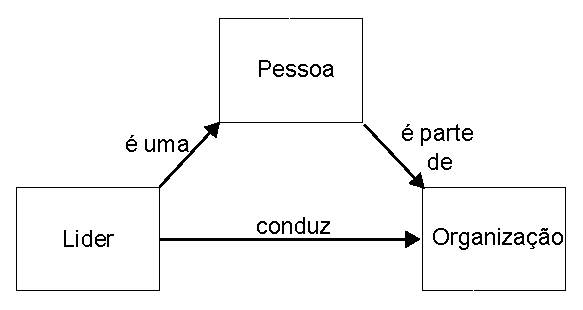
\includegraphics[width=6cm, height=8cm]{./secoes/solucaoProposta/pics/img/Ontologia.eps}
	\label{FIGURA_ONTOLOGIA_CONSTRUIDA}
	\vspace{0.1cm}
	\source{\varAutorData}
\end{figure}

A ontologia construída pode ser visualizada na figura \ref{FIGURA_ONTOLOGIA_CONSTRUIDA}, na qual os círculos são os conceitos do domínio e as linhas de ligação, são as relações entre conceitos. A relação que foi utilizada é a ``\emph{é subtipo de}''. Ao término da fase de construção, foi realizada a fase de validação da ontologia, realizada por um especialista no domínio de bioinformática. Que é orientador deste projeto, tem formação específica em bioinformática e \emph{workflows} científicos. A documentação da ontologia, que é a última etapa, foi realizada nesta seção da dissertação, na qual foram detalhados os motivos de sua construção, sua motivação, seus usos e a forma de sua validação.

\section{Modelagem dos dados}\label{SEC_MODELAGEM} 
Os \emph{workflows} foram obtidos no repositório \emph{myExperiment} \cite{ROURE2015}, por meio do \emph{software wget} \cite{wget2015}. Após efetuar o \emph{download} dos \(2481\) \emph{workflows} em formato \emph{xml}, foi utilizado o analisador de código \emph{Beautiful Soup} \cite{BeautifulSoup2015}, para organizar o conjunto de dados em uma base de dados relacional\footnote{www.each.usp.br/digiampietri/baseworkflows/SQL.tar.gz} (ver figura \ref{figura_modelo_conceitual}).
\begin{figure}[!hbt]
    \centering  
    \caption{Modelo de dados dos \emph{workflows} científicos}
    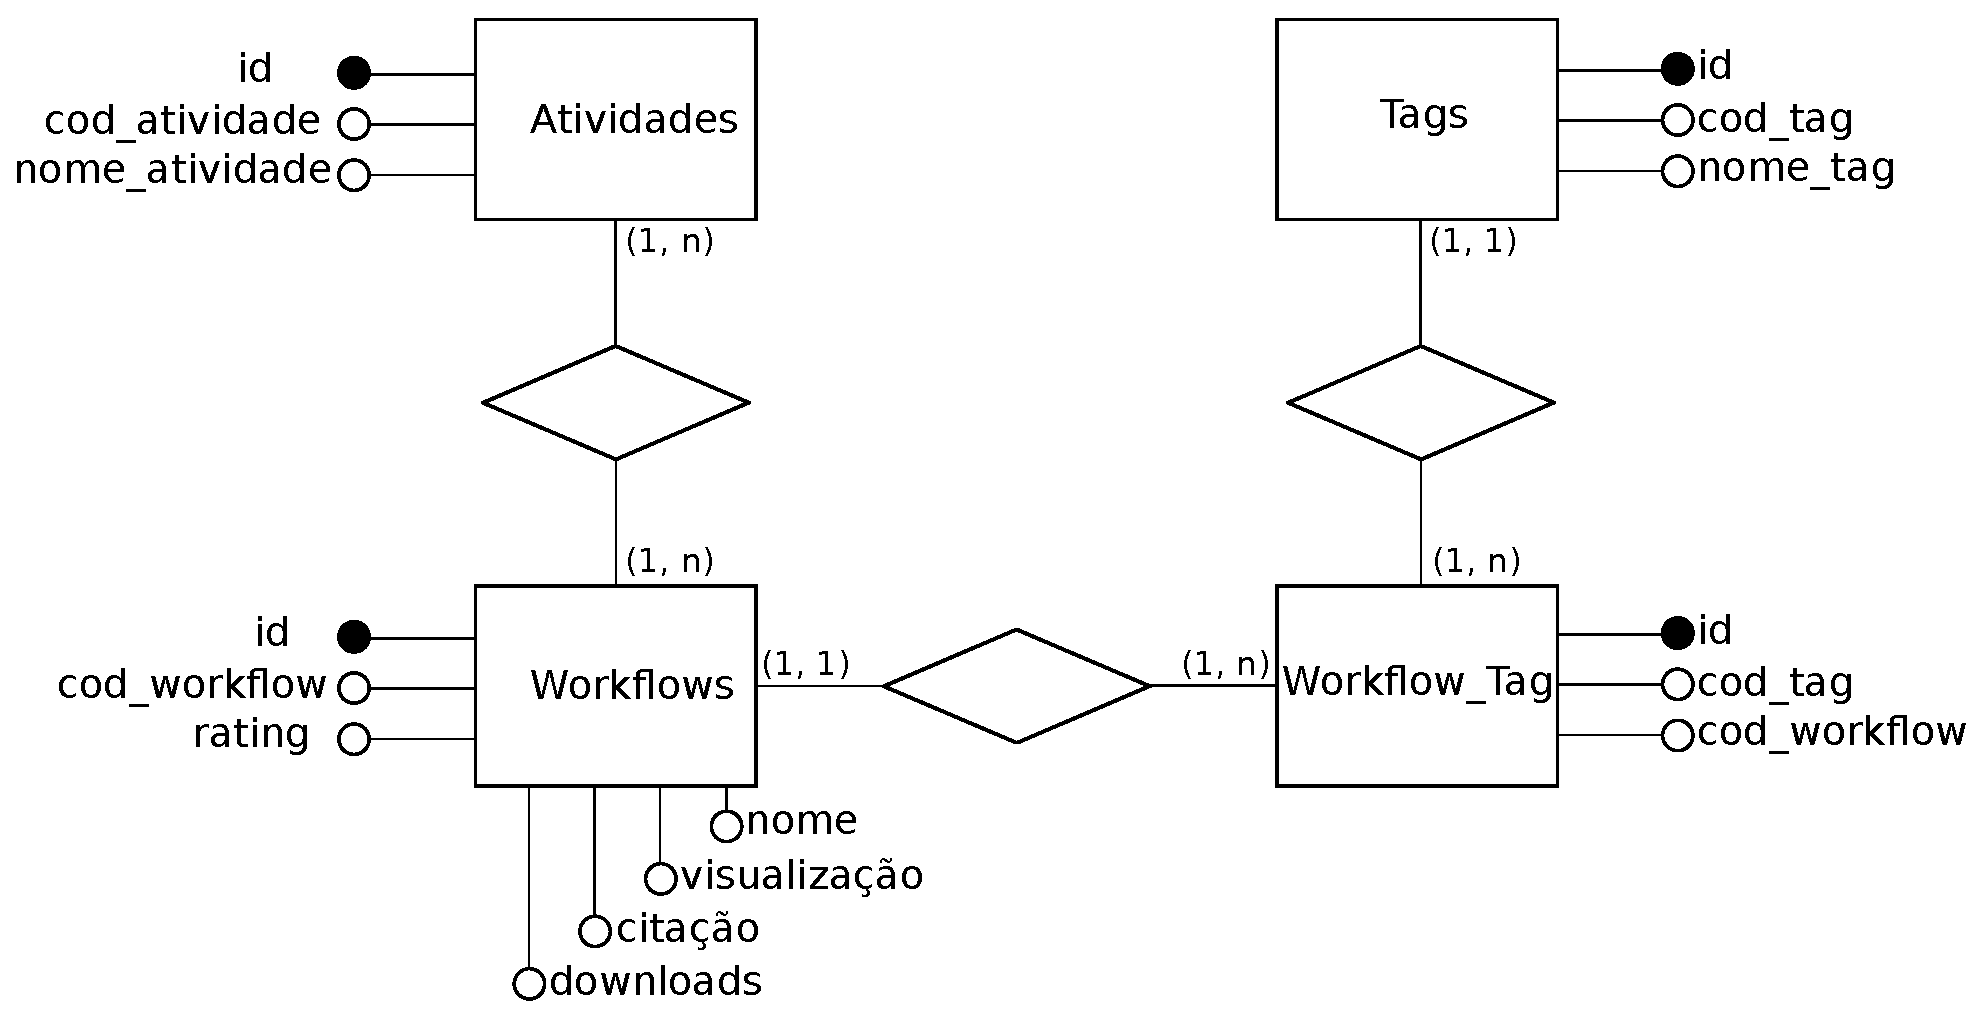
\includegraphics[width=10cm, height=4.5cm]{./secoes/solucaoProposta/pics/img/modelo_conceitual.eps}
    \label{figura_modelo_conceitual}
	\vspace{0.1cm}
    \source{\varAutorData}
\end{figure}
Neste modelo conceitual os retângulos representam as entidades, os losangos representam a relação entre atividades, os círculos brancos representam os atributos das entidades, os círculos pretos representam identificadores e os números próximos a cada entidade representam sua cardinalidade. Este modelo armazena todas as atividades dos \emph{workflows} (de diversas áreas) usando as entidades \emph{Atividades} e \emph{Workflow}. Para registrar qual a área científica (domínio de aplicação) de cada \emph{workflow} foram utilizadas as tabelas \emph{Workflow\_Tag} e \emph{Tag}.

Os \emph{workflows} da área de bioinformática (totalizando \(73\)) em conjunto com suas atividades (totalizando \(280\)) foram convertidos em uma matriz \(M_{i,j}\) em que cada linha \(i\) representa um \emph{workflow}, cada coluna \(j\) representa uma das \(280\) atividades e cada célula da matriz \(M\) representa a existência \(M_{i,j} = 1\), ou não \(M_{i,j} = 0\), da atividade da coluna \(j\) no \emph{workflow} \(i\). A tabela \ref{tabela_matriz_de_dados} apresenta um exemplo, fictício, de matriz \(M\). Para a realização dos testes, para cada linha da tabela \ref{tabela_matriz_de_dados} é removida uma atividade e é recomendada uma lista de possíveis atividades. O objetivo do sistema de recomendação é identificar corretamente qual a atividade está faltando no workflow (isto é, aquela que foi removida). 
\begin{table}[htb]
	\centering
	\caption{Exemplo de matriz de entrada.}
		\begin{tabular}{|c|c|c|c|c|}  \hline
		\textbf{\emph{Workflow}} & \textbf{Ativ \(\mathbf{01}\)} & \textbf{Ativ \(\mathbf{02}\)} & \textbf{\(\mathbf{\ldots}\)} & \textbf{Ativ \(\mathbf{280}\)}  \\ \hline
		01 			  & 1 			  & 0 			  & \(\ldots\) 	  & 0  				\\ \hline
		02 			  & 1 			  & 1 			  & \(\ldots\) 	  & 1  				\\ \hline
		03 			  & 1 			  & 0 			  & \(\ldots\) 	  & 1  				\\ \hline
		\(\vdots\) 		  			  & \(\vdots\) 	  & \(\vdots\) 	  & \(\vdots\) 	  & \(\vdots\) 		\\ \hline
		73 			  & 1 			  & 0 			  & \(\ldots\) 	  & 0  				\\ \hline
		\end{tabular}
	\label{tabela_matriz_de_dados}
	\vspace{0.1cm}
	\source{\varAutorData}
\end{table}

\section{Modelagem dos dados como problema de classificação e regressão}\label{SEC_MODELAGEM_CLASSIFICACAO_REGRESSAO} 
Para usar técnicas de classificação e regressão foram propostas algumas alterações no conjunto de dados original, descrito na tabela \ref{tabela_matriz_de_dados}, as quais podem ser visualizadas na tabela \ref{tabela_matriz_de_dados_adapatada_classificacao_regressao}. Cada \emph{workflow} foi replicado \(118\) vezes. Destes, \(59\) são uma cópia idêntica ao original, enquanto que dos outros \(59\) foi removida uma mesma atividade para todos os \emph{workflows}, e foi adicionada uma nova atividade representando uma possível recomendação. Dessa forma, para cada \emph{workflow} original haverá \(59\) instâncias corretas e \(59\) instâncias incorretas e este tipo de informação será utilizada para treinar os classificadores ou regressores.
\begin{table}[!htb]
	\tiny
	\centering
	\caption{Exemplo de matriz de entrada para técnicas de classificação e regressão}
	\begin{tabular}{|c|c|c|c|c|c|c|c|c|}  \hline
\textbf{\(\#\)} & \textbf{\emph{Workflow}} & \textbf{Ativ \(\mathbf{01}\)} & \textbf{Ativ \(\mathbf{02}\)} & \textbf{\(\mathbf{\ldots}\)}  & \textbf{Ativ \(\mathbf{279}\)} & \textbf{Ativ \(\mathbf{280}\)} & \textbf{Rótulo} \\ \hline

1	&		01		 			   & 1 			  & 0 			  & \(\ldots\) 	  & 0 & 0  			& T	\\ \hline
2	&		01 					   & 1 			  & 0 			  & \(\ldots\) 	  & 0 & 0  			& T	\\ \hline
\(\vdots\)  &  \(\vdots\) 	   	   & \(\vdots\)   & \(\vdots\) 	  & \(\vdots\) 	  & \(\vdots\) & \(\vdots\) & \(\vdots\)\\ \hline
59	&		01 					   & 1 			  & 0 			  & \(\ldots\) 	  & 0 & 0   		& T	\\ \hline
1	&		01		 			   & 0 (removida) 		  & 1 (adicionada) &\(\ldots\)& 1 & 0	& F	\\ \hline
2	&		01 					   & 0 (removida)& 0 		  & \(\ldots\) 	  & 1 (adicionada) & 0& F	\\ \hline
\(\vdots\)  &		\(\vdots\) 	   & \(\vdots\) & \(\vdots\) 	  & \(\vdots\) 	  & \(\vdots\) & \(\vdots\) & \(\vdots\) \\ \hline
59	&		01 					   & 0 (removida)			  & 0 			  & \(\ldots\) & 0 & 1 (adicionada)& F \\ \hline
					&\(\vdots\) & & & & & & 																		\\ \hline
1	&		73		 			   & 1 			  & 1  & \(\ldots\) 	  & 0 & 0  			& T	\\ \hline
2	&		73 					   & 1 			  & 1  & \(\ldots\) 	  & 0 & 0  			& T	\\ \hline
\(\vdots\)  &		\(\vdots\) 	   & \(\vdots\)   & \(\vdots\) 	  & \(\vdots\) 	  & \(\vdots\) & \(\vdots\) & \(\vdots\) \\ \hline
59	&		73 					   & 1 			  & 1  & \(\ldots\) 	  & 0 & 0   		& T	\\ \hline
1	&		73		 			   & 1 (adicionada) & 0 (removida)  & \(\ldots\) 	  & 1 & 0   		& F	\\ \hline
2	&		73 					   & 1 			  & 0 (removida)  & \(\ldots\)& 1 (adicionada) & 0  & F	\\ \hline
\(\vdots\)  &		\(\vdots\) 	   & \(\vdots\)   & \(\vdots\) 	  & \(\vdots\) 	  & \(\vdots\) & \(\vdots\) & \(\vdots\)	\\ \hline
59	&		73 					   & 1 			  & 0 (removida)  & \(\ldots\) 	  & 0 & 1 (adicionada) & F	\\ \hline
		\end{tabular}
	\label{tabela_matriz_de_dados_adapatada_classificacao_regressao}
	\vspace{0.1cm}
	\source{\varAutorData}
\end{table}

A escolha de \(59\) atividades a serem recomendadas foi feita por duas razões. A primeira é selecionar as 59 atividades com maior frequência na base de dados. A segunda é a limitação computacional: replicar as \(280\) possíveis recomendações poderia ser inviável em termos de treinamento. Foram replicadas \(59\) instâncias de \emph{workflows} idênticas consideradas corretas, isto é com a atividade correta não removida, para garantir o balanceamento entre classes. A última alteração foi adicionar uma coluna indicando se a recomendação da atividade proposta é a correta, isto é, a pertencente ao respectivo \emph{workflow} (\emph{T}) ou não (\emph{F}).

Na primeira modelagem, descrita na tabela \ref{tabela_matriz_de_dados}, cada linha (instância) recebe uma lista de atividades recomendadas pelas técnicas da literatura correlata e pela técnica proposta nesse mestrado (seção \ref{SEC_HIBRIDA_PROPOSTA}). Cada lista retornada segue algum critério de ordenação referente à técnica usada. Por exemplo, uma técnica baseada em frequência retorna uma lista de atividades ordenadas pelas suas frequências. 

Na segunda modelagem, cada linha classificada como \emph{não pertencente} (\emph{F}) ao \emph{workflow} é automaticamente adicionada no final da lista de recomendação. As outras atividades (\emph{T}) são adicionadas ao início da lista e ordenadas, de acordo com suas frequências, anotações ontológicas, ordem alfabética e seletor aleatório, nesta sequência de ordenações estáveis.

Esta modelagem foi utilizada pelos classificadores e regressores descritos no capítulo \ref{CAP_CONCEITOS_FUNDAMENTAIS}. Adicionalmente, os resultados desses classificadores e regressores foram utilizados pelo classificador composto e pelo \emph{ensemble} de classificadores. Essas estratégias que utilizam classificadores e regressores foram desenvolvidos de forma a não necessitarem de anotações semânticas dos \emph{workflows}.

Em ambas as modelagens, após construir a lista de recomendação oficial, aquela com os itens recomendados pelas técnicas, os sistemas de recomendação adicionam todas as outras atividades (que não foram recomendadas), ordenadas alfabeticamente, no final da lista. Dessa forma, todas as possíveis atividades estarão presentes na lista. Portanto as métricas descritas na seção \ref{SEC_METRICAS_VALIDACAO} sempre poderão ser calculadas.

\section{Estratégia de validação dos sistemas de recomendação} \label{SEC_METRICAS_VALIDACAO}
Para a validação será utilizada a técnica cruzada considerando \(10\) subconjuntos (\emph{\(10\)-fold cross validation}). Nessa técnica, o conjunto de dados é dividido em 10 subconjuntos (\emph{folds}) e são realizadas dez execuções. Em cada uma, \(10\%\) dos \emph{workflows} são separados para teste e \(90\%\) para treinamento. Assim, para cada execução, o sistema treina com \(90\%\) dos dados e o resultado do treinamento é testado para os \(10\%\) restantes. 

Deve-se ressaltar que \(100\%\) do conjunto de dados é rotulado (isto é, fica explícito ao sistema qual atividade foi removida) e assim é possível verificar o desempenho de cada uma das execuções. O teste apresenta os \(10\%\) de \emph{workflows}, sem informar os rótulos (a atividade removida), para os sistemas de recomendação que já foram treinados. Ao término das dez execuções são calculadas as médias das métricas: i) \emph{Sucess at rank k} (\(S@k\)); e ii) \emph{Mean Reciprocal Rank} (MRR). A figura~\ref{figura_10_fold_cross_validation} ilustra o processo de separação entre conjunto de treinamento e teste utilizado na estratégia de validação empregada.
\begin{figure}[!hbt]
	\centering   
	\caption{Exemplo de \emph{$10$-fold cross validation}}
	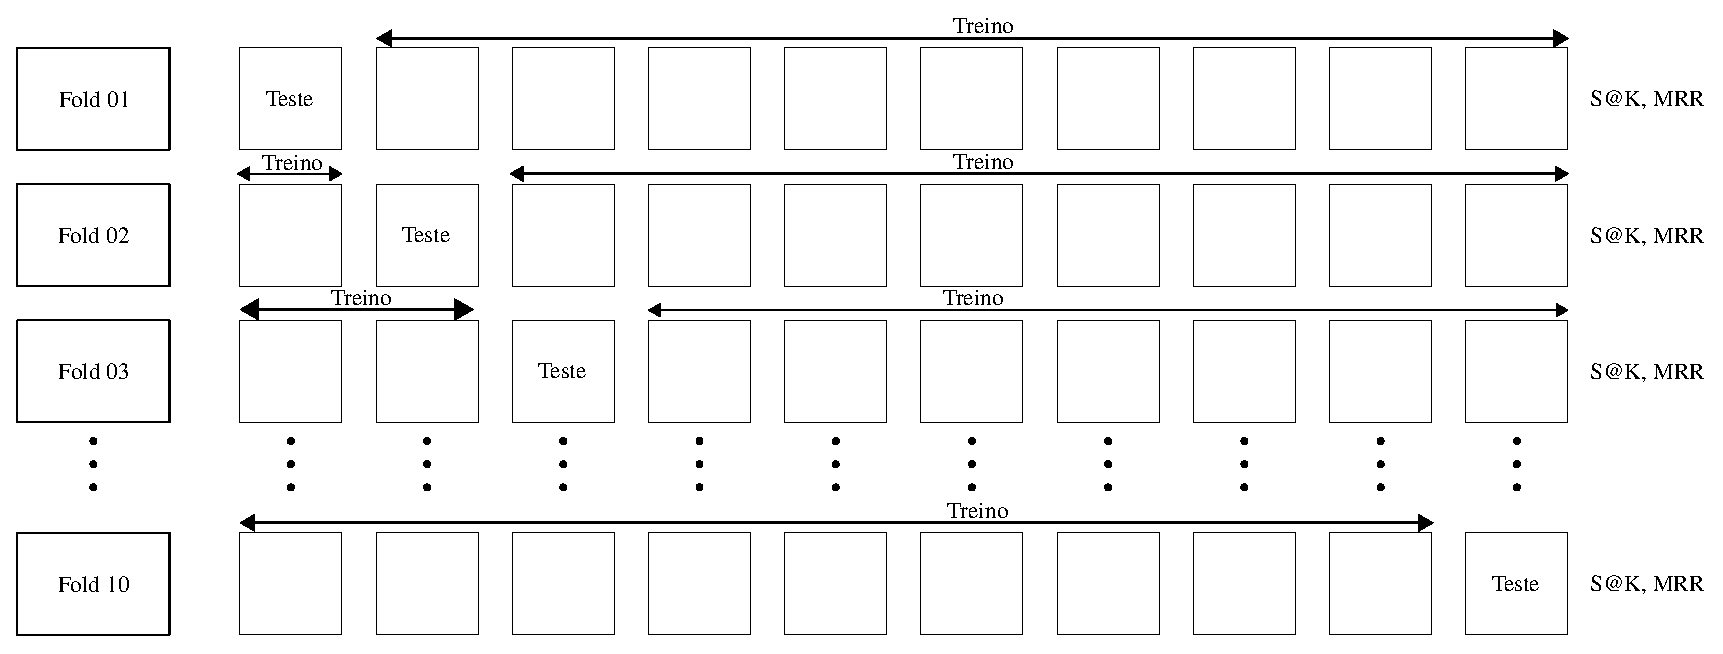
\includegraphics[width=14cm, height=9cm]{./secoes/conceitosFundamentais/pics/img/10FOLDCROSS.eps}
	\vspace{0.1cm}
	\source{Adaptado de \citeonline{HanKamber2011}}
	\label{figura_10_fold_cross_validation}
\end{figure}

A métrica \(S@k\) calcula a probabilidade de um item de interesse estar localizado entre as \(k\) primeiras posições da lista de atividades recomendadas. Seus valores residem entre zero e um. Os resultados dessa métrica são cumulativos para valores crescentes de \(k\), isto ocorre pois se uma atividade de interesse estiver entre as cinco primeiras posições da lista de recomendações, ela também encontra-se entre as dez primeiras posições. No limite, a atividade sempre estará entre as \(L\) primeiras posições, sendo \(L\) o tamanho total da lista de recomendações. Assim, valores elevados para $S@k$ são considerados bons, especialmente para valores baixos de $k$. O cálculo dessas métricas é detalhado pelas equações \cite{Harvey2010}:
\begin{align}
MRR &= \frac{1}{N} \sum\limits_{i=1}^{N} \left( \frac{1}{n_{i}} \right) 		\label{equ_mrr}\\
S@k &= \frac{1}{N} \sum\limits_{i=1}^{N} \left( I(n_{i} \leq k) \right)			\label{equ_s@k}
\end{align}
em que \(N\) é o número de listas recomendadas, \(n_{i}\) é a posição do item desejado na lista de recomendações \(i\), \(k\) é uma posição da lista determinada como parâmetro de entrada da equação \eqref{equ_s@k} e a função \emph{I}, indica se a atividade \(n_{i}\) ocorre em uma posição (\(x\)) menor ou igual ao parâmetro de entrada \(k\), e é dada por
\begin{align}
I(x, k)   &= \begin{cases} \label{equ_indicativa}
1 \textrm{ se } x \leq k \\
0 \textrm{ caso contrário }
\end{cases}
\end{align}

Para exemplificar o uso destas métricas será utilizado um \emph{workflow} fictício representado na figura \ref{figura_atividades_removidas} que teve quatro atividades removidas (\textbf{B}, \textbf{C}, \textbf{A} e \textbf{Z}) uma a uma gerando quatro casos que necessitam de recomendações (\(\mathbf{1}, \mathbf{2}, \mathbf{3}\) e \(\mathbf{4}\)). Que foram usados como entradas para quatro sistemas de recomendação distintos. Cada sistema produziu quatro listas de recomendação, uma para cada caso da figura \ref{figura_atividades_removidas}, rotulados com a mesma numeração. Assim, a lista \(01\) é a recomendação correspondente do caso \(1\) e assim sucessivamente.
\begin{figure}[!hbt]
	\centering   
	\caption{Quatro casos de recomendação de atividades}
	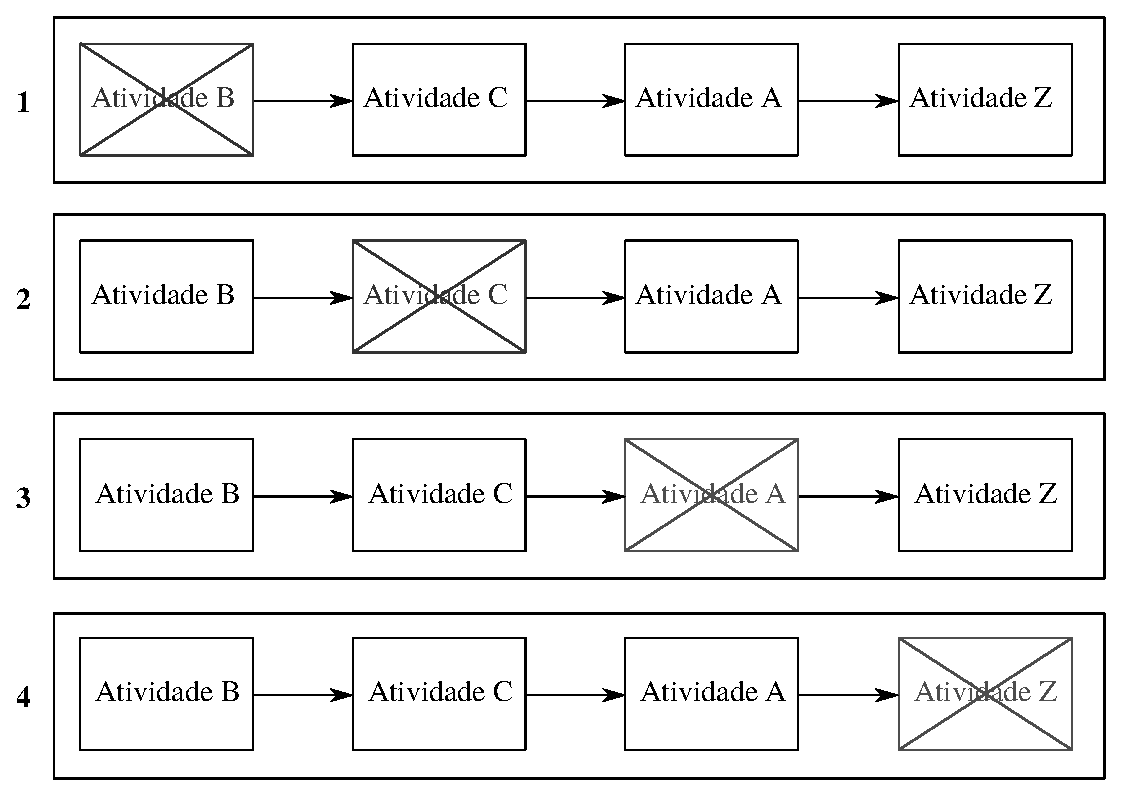
\includegraphics[width=13cm, height=7cm]{./secoes/conceitosFundamentais/pics/img/atividadeRemovida.eps}
	\vspace{0.1cm}
	\source{\varAutorData}
	\label{figura_atividades_removidas}
\end{figure}

As tabelas \ref{TABELAO:SISTEMA_RECOMENDACAO_01}, \ref{TABELAO:SISTEMA_RECOMENDACAO_02}, \ref{TABELAO:SISTEMA_RECOMENDACAO_03} e \ref{TABELAO:SISTEMA_RECOMENDACAO_04} apresentam os resultados dos quatro sistemas de recomendação. Cada item em negrito das listas representa a atividade que foi removida do \emph{workflow}, que é o item considerado correto (atividades com \emph{X} na figura \ref{figura_atividades_removidas}). Sua posição é determinada na coluna \emph{Rank} dessas tabelas.
\begin{table}[!htb]
	\tiny
	\caption{Exemplo de sistemas de recomendações de atividades}
	\begin{subtable}{.5\linewidth}
		\centering
		\begin{tabular}{|c|l|l|l|l|} \hline 
			\textbf{Rank} & \textbf{Lista} \(\mathbf{01}\) & \textbf{Lista} \(\mathbf{02}\) & \textbf{Lista} \(\mathbf{03}\) & \textbf{Lista} \(\mathbf{04}\) \\ \hline 
			1                & Ativ\_A	     		& Ativ\_H    			& Ativ\_Z   		& Ativ\_I    		\\
			2                & \textbf{Ativ\_B}		& Ativ\_B   			& Ativ\_E   		& Ativ\_C 			\\
			3                & Ativ\_C    			& Ativ\_I    			& \textbf{Ativ\_A}  & Ativ\_Z  			\\
			4                & Ativ\_D   			& Ativ\_X    			& Ativ\_X    		& Ativ\_B			\\
			5                & Ativ\_E   			& Ativ\_A			 	& Ativ\_C    		& Ativ\_S			\\
			6                & Ativ\_F   			& Ativ\_D    			& Ativ\_D    		& Ativ\_N			\\
			7                & Ativ\_G   			& \textbf{Ativ\_C}  	& Ativ\_Q    		& Ativ\_K			\\
			8                & Ativ\_H   			& Ativ\_Z    			& Ativ\_B   		& \textbf{Ativ\_Z}	\\
			9                & Ativ\_I    			& Ativ\_P   			& Ativ\_F   		& Ativ\_H			\\
			10               & Ativ\_Z   			& Ativ\_F    			& Ativ\_K    		& Ativ\_A			\\ \hline
		\end{tabular}
		\caption{Sistema de recomendação \(01\)}   
		\label{TABELAO:SISTEMA_RECOMENDACAO_01}		
	\end{subtable}%
	\begin{subtable}{.5\linewidth}
		\centering
		\begin{tabular}{|c|l|l|l|l|} \hline 
			\textbf{Rank} & \textbf{Lista} \(\mathbf{01}\) & \textbf{Lista} \(\mathbf{02}\) & \textbf{Lista} \(\mathbf{03}\) & \textbf{Lista} \(\mathbf{04}\) \\ \hline 
			1                & Ativ\_A	     		& \textbf{Ativ\_C}		& \textbf{Ativ\_A}	& Ativ\_I                    \\
			2                & \textbf{Ativ\_B} 	& Ativ\_B   			& Ativ\_E   		& Ativ\_C 	                 \\
			3                & Ativ\_C    			& Ativ\_I    			& Ativ\_Z			& Ativ\_A                    \\
			4                & Ativ\_D   			& Ativ\_X    			& Ativ\_X    		& \textbf{Ativ\_Z}           \\
			5                & Ativ\_E			   	& Ativ\_A			  	& Ativ\_C    		& Ativ\_S	                 \\
			6                & Ativ\_F   			& Ativ\_D    			& Ativ\_D    		& Ativ\_N                    \\
			7                & Ativ\_G   			& Ativ\_H    			& Ativ\_Q    		& Ativ\_K	                 \\
			8                & Ativ\_H   			& Ativ\_Z    			& Ativ\_B   		& Ativ\_U	                 \\
			9                & Ativ\_I    			& Ativ\_P   			& Ativ\_F   		& Ativ\_H	                 \\
			10               & Ativ\_Z   			& Ativ\_F    			& Ativ\_K    		& Ativ\_X	           \\ \hline
		\end{tabular}
		\caption{Sistema de recomendação \(02\)}
		\label{TABELAO:SISTEMA_RECOMENDACAO_02}
	\end{subtable}
	\\ \\ \hfill 
	\begin{subtable}{.5\linewidth}
		\centering
		\begin{tabular}{|c|l|l|l|l|} \hline 
			\textbf{Rank} & \textbf{Lista} \(\mathbf{01}\) & \textbf{Lista} \(\mathbf{02}\) & \textbf{Lista} \(\mathbf{03}\) & \textbf{Lista} \(\mathbf{04}\) \\ \hline 
			1                & Ativ\_A			    & Ativ\_H    			& Ativ\_F   		& Ativ\_I                    \\
			2                & Ativ\_G    			& Ativ\_B   			& Ativ\_E   		& Ativ\_C 	                 \\
			3                & Ativ\_C    			& Ativ\_I    			& Ativ\_Z			& Ativ\_A                    \\
			4                & Ativ\_D   			& Ativ\_X    			& Ativ\_X    		& Ativ\_B	                 \\
			5                & Ativ\_E   			& Ativ\_A	  			& Ativ\_C    		& Ativ\_S	                 \\
			6                & Ativ\_F   			& Ativ\_D    			& Ativ\_D    		& Ativ\_N                    \\
			7                & \textbf{Ativ\_B}		& Ativ\_Q				& Ativ\_Q    		& \textbf{Ativ\_Z}           \\
			8                & Ativ\_H   			& Ativ\_Z    			& Ativ\_B   		& Ativ\_U	                 \\
			9                & Ativ\_I    			& Ativ\_P   			& \textbf{Ativ\_A}	& Ativ\_H	                 \\
			10               & Ativ\_Z   			& \textbf{Ativ\_C}		& Ativ\_K    		& Ativ\_X           \\ \hline
		\end{tabular}
		\caption{Sistema de recomendação \(03\)}
		\label{TABELAO:SISTEMA_RECOMENDACAO_03}
	\end{subtable}%
	\begin{subtable}{.5\linewidth}
		\centering
		\begin{tabular}{|c|l|l|l|l|} \hline 
			\textbf{Rank} & \textbf{Lista} \(\mathbf{01}\) & \textbf{Lista} \(\mathbf{02}\) & \textbf{Lista} \(\mathbf{03}\) & \textbf{Lista} \(\mathbf{04}\) \\ \hline 
			1                & Ativ\_A			    & Ativ\_H    			& Ativ\_Z   		& \textbf{Ativ\_Z}           \\
			2                & Ativ\_Z    			& \textbf{Ativ\_C}		& Ativ\_E   		& Ativ\_C 	                 \\
			3                & Ativ\_C    			& Ativ\_I    			& Ativ\_Z			& Ativ\_A                    \\
			4                & Ativ\_D   			& Ativ\_X    			& Ativ\_X    		& Ativ\_B	                 \\
			5                & Ativ\_E   			& Ativ\_A			  	& Ativ\_C    		& Ativ\_X 	         		 \\
			6                & Ativ\_F   			& Ativ\_D    			& Ativ\_D    		& Ativ\_N                    \\
			7                & Ativ\_G   			& Ativ\_C    			& Ativ\_Q    		& Ativ\_K	                 \\
			8                & Ativ\_H   			& Ativ\_Z    			& Ativ\_B   		& Ativ\_U	                 \\
			9                & Ativ\_I    			& Ativ\_P   			& \textbf{Ativ\_A}	& Ativ\_H	                 \\
			10               & \textbf{Ativ\_B}  	& Ativ\_F    			& Ativ\_K    		& Ativ\_S		     \\ \hline
		\end{tabular}
		\caption{Sistema de recomendação \(04\)}
		\label{TABELAO:SISTEMA_RECOMENDACAO_04}
	\end{subtable}
	\label{TABELAO}
	\vspace{0.1cm}
	\source{\varAutorData}
\end{table}
O sistema de recomendação \(01\), cujos resultados se encontram na tabela \ref{TABELAO:SISTEMA_RECOMENDACAO_01}, apresenta os seguintes valores de \(S@k\)
\begin{align}
S@1 &= \frac{1}{4}  \Big( (I_{L_{1}} = 0) + (I_{L_{2}} = 0) + (I_{L_{3}} = 0) + (I_{L_{4}} = 0) \Big)	=	0,00	\\
S@3 &= \frac{1}{4}  \Big( (I_{L_{1}} = 1) + (I_{L_{2}} = 0) + (I_{L_{3}} = 1) + (I_{L_{4}} = 0) \Big)	=	0,50	\\
S@5 &= \frac{1}{4}  \Big( (I_{L_{1}} = 1) + (I_{L_{2}} = 0) + (I_{L_{3}} = 1) + (I_{L_{4}} = 0) \Big)	=	0,50	\\
S@7 &= \frac{1}{4}  \Big( (I_{L_{1}} = 1) + (I_{L_{2}} = 1) + (I_{L_{3}} = 1) + (I_{L_{4}} = 0) \Big)	=	0,75	\\
S@10 &= \frac{1}{4} \Big( (I_{L_{1}} = 1) + (I_{L_{2}} = 1) + (I_{L_{3}} = 1) + (I_{L_{4}} = 1) \Big) 	=	1,00		
\end{align}
sendo \(I_{L_{1}}\) o resultado da função indicadora \eqref{equ_indicativa}. As posições das atividades recomendadas por sistema são
\begin{align}
\left( \frac{1}{n_{i}} \right)_{L_{1}}  &= \frac{1}{2} 	\\
\left( \frac{1}{n_{i}} \right)_{L_{2}} &= \frac{1}{7} 	\\
\left( \frac{1}{n_{i}} \right)_{L_{3}} &= \frac{1}{3} 	\\
\left( \frac{1}{n_{i}} \right)_{L_{4}} &= \frac{1}{8} 	
\end{align}
e cuja média é dada por
\begin{align}
MRR &= \frac{\left( \frac{1}{2} + \frac{1}{7} + \frac{1}{3} + \frac{1}{8} \right)}{4} = 0,275297
\end{align}
De forma análoga os resultados obtidos pelos sistemas \(02\), \(03\) e \(04\) podem ser visualizados na tabela \ref{tabela_resultados_mrr_Sak}.
\begin{table}[!htb]
	\centering
	\caption{Lista de recomendação ordenada por frequência}
	\begin{tabular}{ccccccc} \hline
		\textbf{Sistema} & \(\mathbf{S@1}\) & \(\mathbf{S@3}\) & \(\mathbf{S@5}\) & \(\mathbf{S@7}\) & \(\mathbf{S@10}\) & \textbf{MRR}	\\ \hline
		1 & \(0,00\) 	& \(0,50\)	& \(0,50\)	& \(0,75\)	& \(1,00\) & \(0,275297\) \\ 
		2 & \(0,50\)	& \(0,75\)	& \(1,00\)	& \(1,00\)	& \(1,00\) & \(0,687500\) \\ 
		3 & \(0,00\)	& \(0,00\)	& \(0,00\)	& \(0,50\)	& \(1,00\) & \(0,124206\) \\ 
		4 & \(0,25\)	& \(0,50\)	& \(0,50\) 	& \(0,50\)	& \(1,00\) & \(0,427777\) \\ \hline
	\end{tabular}
	\label{tabela_resultados_mrr_Sak}
	\vspace{0.1cm}
	\source{\varAutorData}
\end{table}

Ao comparar os quatro sistemas é possível constatar que, de acordo com as métricas calculadas, o melhor é o número~\(02\) pois apresenta o maior valor de \(MRR = 0,687500\) e os maiores valores observados de \(S@1 = 0,50\) e \(S@3 = 0,75\).


\section{Solução híbrida de frequência e ontologia de domínio}\label{SEC_HIBRIDA_PROPOSTA} 
Uma outra solução proposta neste mestrado recomenda atividades usando três conceitos importantes na área de \emph{workflows} científicos: i) frequência de atividades; ii) compatibilidade entre entrada e saída; e ii) semântica de atividades. Para explicar esta proposta, será usada a figura \ref{FIGURA_ONTOLOGIA_CONSTRUIDA2} como exemplo. Nela é possível observar seis \emph{workflows} com suas anotações, que simulam uma base de dados de \emph{workflows} científicos.
\begin{figure}[!hbt]
	\centering
 	\caption{Exemplo de banco de dados de \emph{workflows} científicos}
		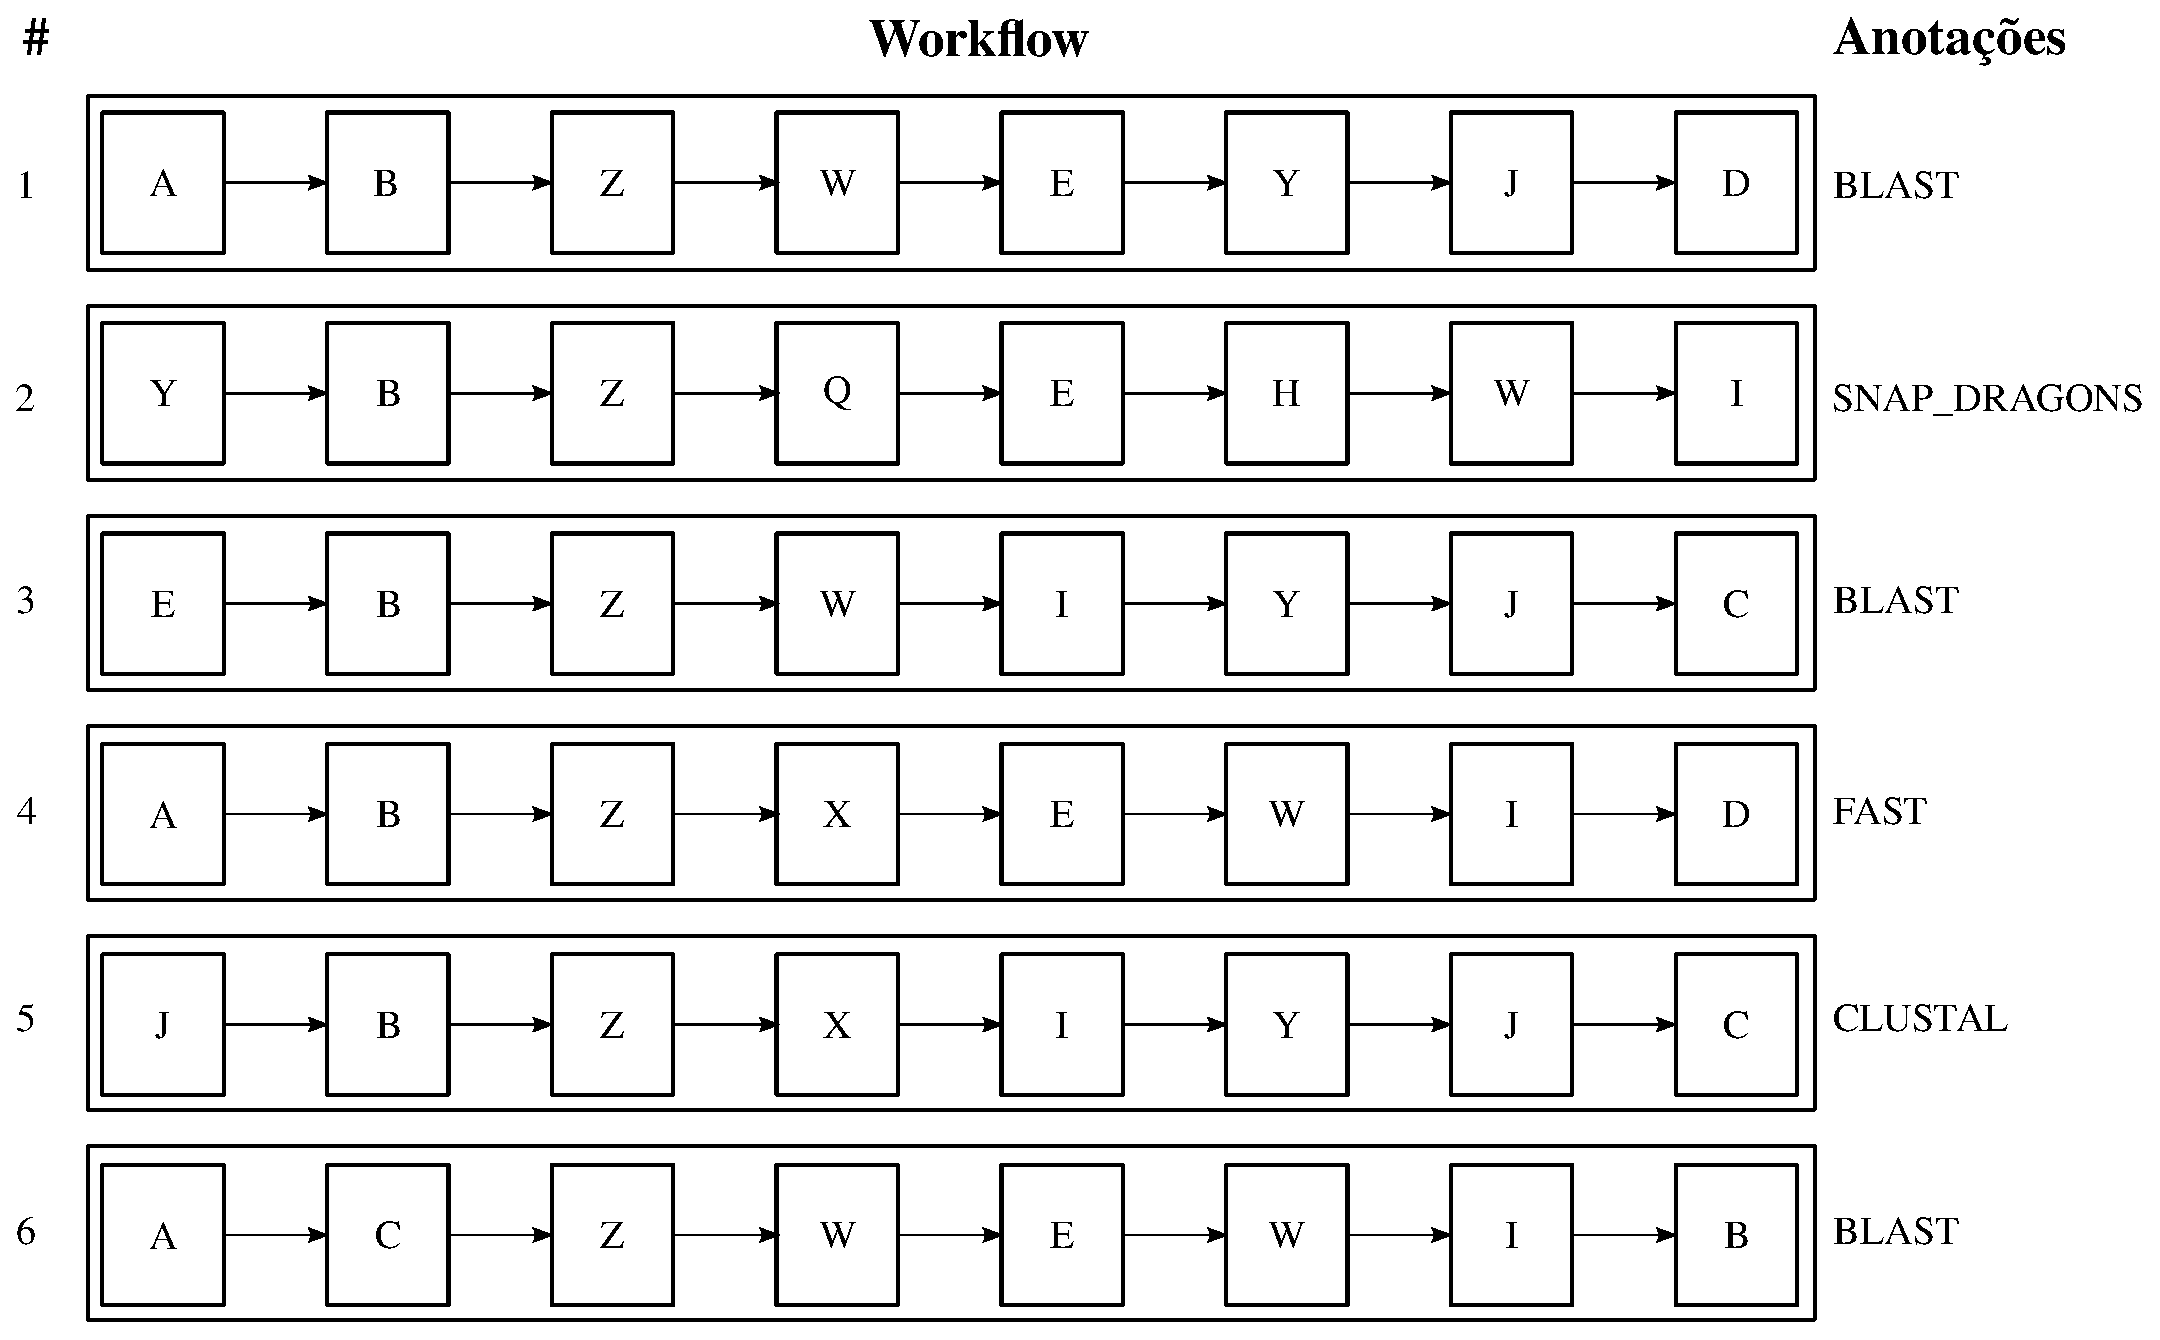
\includegraphics[width=12cm, height=7cm]{./secoes/solucaoProposta/pics/img/recomendacaofreqontologia.eps}
	\label{FIGURA_ONTOLOGIA_CONSTRUIDA2}
	\source{\varAutorData}
\end{figure}

A solução proposta começa calculando a frequência de ocorrência de cada par de atividades existentes, que é o número de vezes que uma atividade \emph{W} ocorre imediatamente após uma outra atividade \emph{Z}. Ao considerar somente atividades que já foram conectadas, previamente na base de \emph{workflows}, a compatibilidade de entrada e saída é garantida por consequência.

Após calcular a frequência é necessário anotar todos os \emph{workflows} da figura \ref{FIGURA_ONTOLOGIA_CONSTRUIDA2}, usando os conceitos da ontologia construída (ver figura \ref{FIGURA_ONTOLOGIA_CONSTRUIDA}). Essa etapa é feita manualmente (de forma não automatizada). Por fim, o algoritmo anota todas as atividades com as mesmas anotações de seus respectivos \emph{workflows}; isto é, se a atividade \emph{X} (da figura \ref{FIGURA_ONTOLOGIA_CONSTRUIDA2}) está dentro de dois \emph{workflows} com anotações distintas então esta atividade receberá duas anotações. O resultado final é a tabela \ref{tabela_lista_recomendacao_ordenada_frequencia}, que apresenta as frequências e anotações de atividades, nesse ponto o sistema está treinado e pronto para uso do cientista

Para compreender o mecanismo de recomendação treinado será usado outro exemplo, cujo objetivo é simular a interação do usuário com o sistema de recomendação. Suponha que durante a construção do \emph{workflow} \(1\) (ver figura \ref{FIGURA_ONTOLOGIA_CONSTRUIDA}) um cientista insira a atividade \emph{Z} e solicite uma recomendação. O sistema vai procurar na lista das atividades posteriores a \emph{Z} ordenadas por frequência e conceito ontológico e irá retornar a lista de recomendação apresentada na tabela~\ref{tabela_lista_recomendacao_ordenada_frequencia}. A ordenação por conceito ontológico, além de ser estável serve como critério de desempate, quando duas atividades tiverem a mesma frequência. Neste exemplo, de acordo com a lista de recomendação da tabela~\ref{tabela_lista_recomendacao_ordenada_frequencia}, a atividade \emph{W} seria recomendada em primeiro lugar ao cientista, o que representa um acerto.
\begin{table}[!htb]
	\centering
	\caption{Recomendação para a atividade \emph{Z} ordenada por frequência e conceito ontológico}
		\begin{tabular}{|c|c|c|c|}  \hline
		\textbf{Posição na Lista} & \textbf{Ativ} & \textbf{Frequência} & \textbf{Anotação Atividade} 	\\ \hline
		1				& W 				& 3 				& BLAST				\\ \hline
		2				& X 				& 2 				& FAST, CLUSTAL		\\ \hline
		3				& Q 				& 1 				& SNAP DRAGONS		\\ \hline
		\(\vdots\)		& \(\vdots\)		& \(\vdots\) 		& \(\vdots\)		\\ \hline
		280				& \(\vdots\)		& \(\vdots\)		& \(\vdots\)	\\ \hline
		\end{tabular}
	\label{tabela_lista_recomendacao_ordenada_frequencia}
	\vspace{0.1cm}
	\source{\varAutorData}
\end{table}

As atividades são anotadas com a mesma anotação dos \emph{workflows} que as contém. Dessa forma, é possível que haja pelo menos uma atividade com mais de uma anotação. Isso gera um novo caso de recomendação a ser considerado. Suponha que ambas as atividades \emph{W} e \emph{X} contenham dentro de suas listas de anotação o conceito \emph{BLAST}. Nesse caso, seria recomendada a atividade com menor número de anotações, por ser considerada mais específica para o experimento em questão. Caso ambas as atividades tenham o mesmo número de anotações, é utilizada a ordem alfabética de conceitos como critério de desempate. Se ocorrer um novo empate é usado um seletor aleatório.